\documentclass[11pt]{article}

\usepackage[czech]{babel}
\usepackage{a4wide}
\usepackage[utf8]{inputenc}
\usepackage[T1]{fontenc}
\usepackage{fancyhdr}
\usepackage{amssymb}
\usepackage{amsthm}
\usepackage{amsmath}
\usepackage{mathtools}
\usepackage{mleftright}
\usepackage{subcaption}
\usepackage{gensymb}
\usepackage{parskip}
\usepackage[outputdir=Build]{minted}
\setminted{
frame=lines,
framesep=2mm,
linenos,
autogobble
}

% ---------------------------------------- BIBLIOGRAFIE ----------------------------------------
\usepackage[backend=biber, style=numeric]{biblatex}
\addbibresource{main.bib}

% ---------------------------------------- JEDNOTKY ----------------------------------------
\usepackage{siunitx}
\sisetup{per-mode = symbol}

% ---------------------------------------- FLOATY ----------------------------------------
\usepackage{float}
\floatplacement{figure}{H}

% ---------------------------------------- PŘÍKLADY ----------------------------------------
% https://tex.stackexchange.com/questions/164113/the-exercise-package-in-list-form

\usepackage{scrextend}

\usepackage[load-headings]{exsheets}
\DeclareInstance{exsheets-heading}{mylist}{default}{
  runin = true ,
  attach = {
    main[l,vc]number[l,vc](-2em,0pt) ;
    main[l,vc]title[l,vc](-5.5em,0pt)
  }
}

\DeclareRobustCommand*\questionstar{\texorpdfstring{\bonusquestionsign}{* }}
\DeclareRobustCommand*\bonusquestionsign{\llap{$\bigstar$\space}}

\NewQuSolPair
	{question*}[name=\questionstar Příklad]
	{solution*}[name=\questionstar Řešení]

\DeclareTranslation{Czech}{exsheets-exercise-name}{Příklad}
\DeclareTranslation{Czech}{exsheets-solution-name}{Řešení}

\SetupExSheets{
  headings = mylist , % use the new headings instance
  headings-format = \it ,
  counter-format = se.qu ,
  counter-within = section ,
	question/pre-hook = \addmargin[5.5em]{0em} ,
	solution/pre-hook = \addmargin[5.5em]{0em} ,
	question/post-hook = \endaddmargin ,
	solution/post-hook = \endaddmargin
}

% https://tex.stackexchange.com/questions/263467/exsheets-how-to-get-a-counter-reference-combining-section-and-question-numbers
\renewcommand\thequestion{\thesection.\arabic{question}}

% ------------------------------------------------------------------------------------------

% forcing footnotes to be at the very bottom
\usepackage[bottom]{footmisc}

\usepackage{hyperref}
\urlstyle{same}
\hypersetup{
    colorlinks=true,
    urlcolor=blue,
    linkcolor=black,%TOC
}

\usepackage{titlesec}
\usepackage{subfiles}

\usepackage{geometry}
\geometry{
    a4paper,
    total={170mm,257mm},
    right=20mm,
    left=20mm,
    top=30mm,
    bottom=20mm,
}

% ---------------------------------------- NADPISY ----------------------------------------
\titleformat{\section} {\normalfont\fontsize{16}{15}\bfseries}{\thesection}{1em}{}
\titleformat{\subsection} {\normalfont\fontsize{14}{15}\bfseries}{\thesubsection}{1em}{}
\titleformat{\subsubsection} {\normalfont\fontsize{12}{15}\bfseries}{\thesubsubsection}{1em}{}

\usepackage{tcolorbox}
\tcbset{on line,
        boxsep=4pt, left=0pt,right=0pt,top=0pt,bottom=0pt,
        colframe=white
        }

% ---------------------------------------- HLAVIČKA ----------------------------------------
\pagestyle{fancy}
\fancyhf{}
% Now set the headers
\fancyhead[LE,RO]{\footnotesize\thepage}
\fancyhead[LO,RE]{\footnotesize\leftmark}
\fancyfoot{}
\fancyfoot[R]{\thepage}

% ---------------------------------------- BARVY ----------------------------------------
\definecolor{ceruleanblue}{rgb}{0.16, 0.32, 0.75}
\definecolor{motorlight}{rgb}{0.85, 0.80, 0.70}
\definecolor{motordark}{rgb}{0.64, 0.51, 0.25}
\definecolor{wait}{rgb}{0.64, 0.25, 0.25}


% ---------------------------------------- DOKUMENT ----------------------------------------
\begin{document}


\begin{titlepage}
    \begin{center}
        \vspace*{3em}
% ---------------------------------------- ÚVODNÍ STRÁNKA ----------------------------------------
        \Huge
				\textbf{Úvod do programování} 
\includegraphics[height=0.65\baselineskip]{Images/vex-logo.png}
				\\
				\Large
        \vspace*{0.5em}
				v jazyce Blocky a prostředí RobotMesh studio

        \vfill
				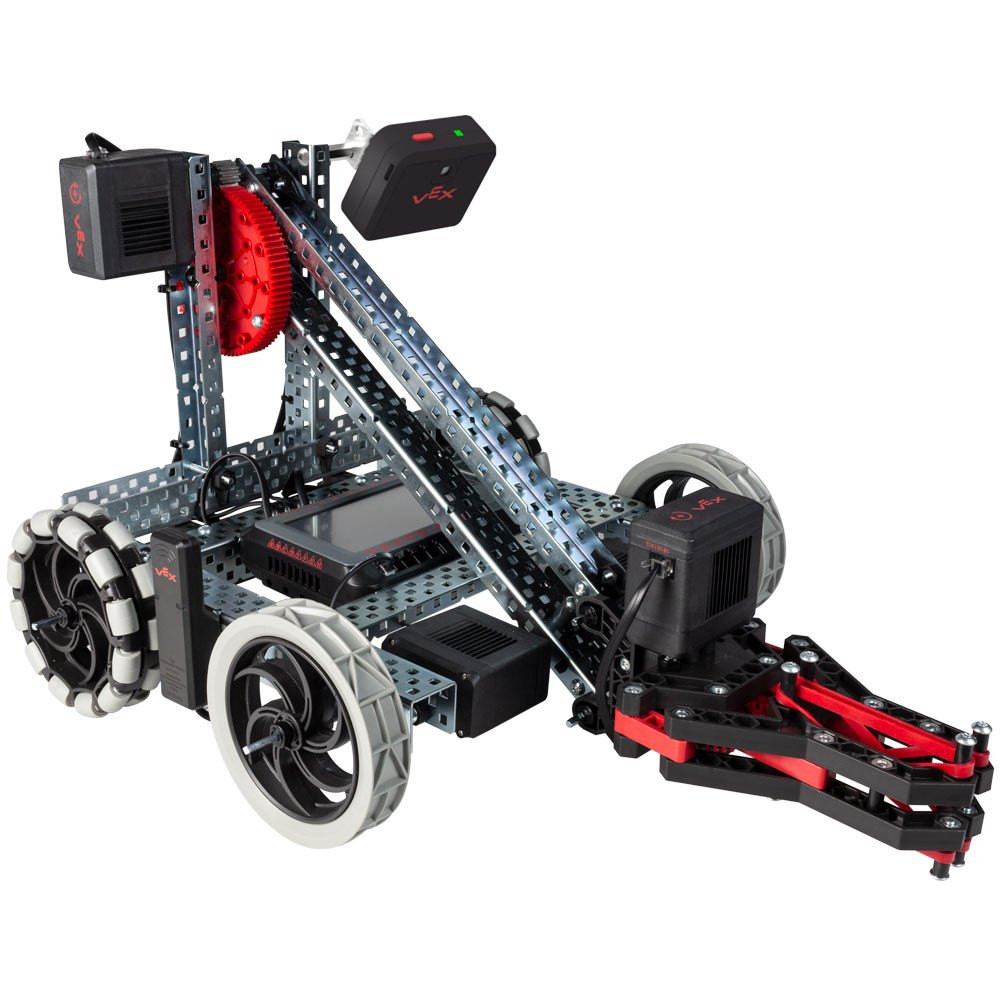
\includegraphics[width=0.7\linewidth]{Images/robot.jpg}
        \vfill

        \flushright
        \normalsize
				Tomáš Sláma\\
				\today
    \end{center}
\end{titlepage}

\tableofcontents
\clearpage

% ---------------------------------------- DEFINICE BLOKŮ ----------------------------------------
\newcommand{\block}{$\vcenter{\hbox{
\includegraphics[height=0.8em]{../Images/blocky-logo.png}}}$}
\newcommand{\centerimage}[2]{$\vcenter{\hbox{\includegraphics[height=#1]{#2}}}$}


\newcommand{\blockMotorStart}{\item[\block] \centerimage{2em}{../Images/blocks/motor-start.png} -- \parbox{0.545\textwidth}{zapne daný motor dopředu (\textit{forward}) nebo dozadu (\textit{reverse}) na danou rychlost (\textit{velocity}) v procentech.}}
\newcommand{\blockMotorStop}{\item[\block] \centerimage{1.6em}{../Images/blocks/motor-stop.png} -- vypne daný motor.}
\newcommand{\blockMotorDistance}{\item[\block] \centerimage{2em}{../Images/blocks/motor-distance-start.png} -- \parbox{0.525\textwidth}{zapne motor, dokud se neotočí o daný počet stupňů (\textit{degrees}) nebo otáček (\textit{revolutions}). Je neblokující -- zapne motor a jde na další block.}}
\newcommand{\blockMotorVelocity}{\item[\block] \centerimage{2em}{../Images/blocks/motor-velocity.png} -- nastaví rychlost motoru, ale nezapne ho!}

\newcommand{\blockMotorDoneImage}{\centerimage{1.6em}{../Images/blocks/motor-done.png} }
\newcommand{\blockMotorDone}{\item[\block] \blockMotorDoneImage -- podmínka která říká, zda daný motor skončil.}

\newcommand{\blockLoop}{\item[\block] \centerimage{4em}{../Images/blocks/loop.png} -- opakuje bloky uvnitř několikrát.}
\newcommand{\blockLoopForever}{\item[\block] \centerimage{4em}{../Images/blocks/loop-forever.png} -- opakuje bloky uvnitř donekonečna.}
\newcommand{\blockLoopWhile}{\item[\block] \centerimage{4em}{../Images/blocks/loop-while.png} -- \parbox{0.725\textwidth}{opakuje bloky uvnitř, dokud (\textit{while}) nebo než (\textit{until}) platí podmínka.}}

\newcommand{\blockWaitImage}{\centerimage{2em}{../Images/blocks/wait.png} }
\newcommand{\blockWait}{\item[\block] \blockWaitImage -- čeká daný čas.}
\newcommand{\blockWaitUntil}{\item[\block] \centerimage{1.6em}{../Images/blocks/wait-until.png} -- čeká, než (\textit{until}) platí podmínka.}
\newcommand{\blockStartImage}{\centerimage{1.6em}{../Images/blocks/start.png} }
\newcommand{\blockStart}{\item[\block] \blockStartImage -- startovní blok pro každý Blocky program.}

\newcommand{\blockFunctionDefinition}{\item[\block] \centerimage{4em}{../Images/blocks/function-definition.png} -- definování funkce; jméno lze upravit kliknutím.}
\newcommand{\blockFunctionCall}{\item[\block] \centerimage{2em}{../Images/blocks/function-call.png} -- volání funkce.}

\newcommand{\blockBumperPressed}{\item[\block] \centerimage{1.6em}{../Images/blocks/bumper-pressed.png} -- podmínka, která říká, zda je daný senzor stisknutý.}

\setcounter{secnumdepth}{0}
\section{Na úvod}
Tato učebnice byla sepsána Tomášem Slámou ke vzdělávacímu programu Robotika 3 TODO (odborněji). Její cíl je seznámit čtenáře s programováním robota VEX V5 za použití programovacích jazyků Blocky a prostředí RobotMesh.

Její aktuální verze je zdarma dostupná na odkazu TODO.

\subsection{Předpoklady}
Učebnice je určena pro naprosté začátečníky, předchozí znalosti robotiky/programování nejsou potřeba.

Většina příkladů předpokládá, že vlastníte sadu TODO a máte postaveného robota TODO. Není problém procházet učebnici bez přesně této sady/postaveného robota, ale je možné, že řešení některých příkladů bude jiné.

\subsection{Příklady}
Každá část učebnice obsahuje příklady na probíranou látku, které vřele doporučuji dělat -- programovací jazyk se není možné naučit čtením učebnice, je potřeba v něm opravdu programovat!

Příklady označené $\bigstar$ jsou časově/nápadově náročnější než ostatní, takže se rozhodně netrapte tím, že by se vám některé z nich nepodařily vyřešit.

Příklady, u kterých to dává smysl, jsou rovněž dostupné v části \nameref{cha:sol} -- pokud se na nějakém problému zaseknete, nebo si prostě nebudete jisti řešením, nebojte se si ho v této části prohlédnout.

\subsection{Chyby, překlepy, doplňky}
Pokud někde odhalíte chybu/překlep, nebo máte pocit, že by něco šlo napsat lépe, tak mě buďto kontaktuje na adrese \href{mailto:tomas@slama.dev}{tomas@slama.dev}, nebo vytvořte issue/pull request na stránce \url{https://github.com/xiaoxiae/uvod-do-programovani-vex-v5}.

\newpage

\setcounter{secnumdepth}{3}
\subfile{Chapters/01.tex}
\newpage
\subfile{Chapters/02.tex}
\newpage
\subfile{Chapters/03.tex}
\newpage
\subfile{Chapters/04.tex}
\newpage
\subfile{Chapters/05.tex}
\newpage
\subfile{Chapters/06.tex}
\newpage
\subfile{Chapters/07.tex}
\newpage
\setcounter{secnumdepth}{0}

\newcommand{\where}[1]{{\normalfont (#1)}}

\section{Přehled bloků}

\subsection{Ovládání motoru \where{VEX V5 Motors}}
\begin{itemize}
	\blockMotorStart
	\blockMotorStop
	\blockMotorDistance
	\blockMotorVelocity
\end{itemize}

\subsection{Smyčky \where{Loops}}
\begin{itemize}
	\blockLoop
	\blockLoopForever
	\blockLoopWhile
\end{itemize}

\subsection{Ostatní \where{Robot Mesh}}
\begin{itemize}
	\blockStart
	\blockMotorDone
	\blockWait
	\blockWaitUntil
\end{itemize}

\subsection{Funkce \where{Functions}}
\begin{itemize}
	\blockFunctionDefinition
	\blockFunctionCall
\end{itemize}

\subsection{Senzory \where{TriPort Inputs}}
\begin{itemize}
	\blockBumperPressed
\end{itemize}

\newpage

\section{Řešení příkladů}\label{cha:sol}

\printsolutions

\newpage

\nocite{*}
\printbibliography[title={Zdroje a odkazy}]
\end{document}
